\documentclass[a4paper]{article}
\usepackage[UTF8]{ctex}
\usepackage{geometry}
\usepackage{graphicx}
\usepackage{url}
\usepackage{multirow}
\usepackage{array}
\usepackage{booktabs}
\usepackage{url}
\usepackage{enumitem}
\usepackage{graphicx}
\usepackage{float}
\usepackage{amssymb}
\usepackage{amsmath}
\usepackage{subfig}
\usepackage{longtable}
\usepackage{pifont}
\usepackage{color}
\usepackage{listings}
\usepackage{xcolor}

\allowdisplaybreaks

\geometry{a4paper, scale=0.78}

% \begin{figure}[H]
%     \centering
%     \includegraphics[width=.55\textwidth]{E.png}
%     \caption{矩阵与列向量的乘法}
%     \label{fig:my_label_1}
% \end{figure}

% \left\{
% \begin{array}{ll}
%       x+2x+z=2 & \\
%       3x+8y+z=12 & \\
%       4y+z=2
% \end{array}
% \right.

% \begin{enumerate}[itemindent = 1em, itemsep = 0.4pt, parsep=0.5pt, topsep = 0.5pt]

% \end{enumerate}

%\stackrel{a}{\longrightarrow}

\title{Probability Graph 03 D-Separation}
\author{Chen Gong}
\date{25 November 2019}

\begin{document}
\maketitle
上一小节中,我们已经大致介绍了概率图之间的三种基本拓扑结构。下面我们来介绍一下,这三种拓扑结构的运用,以及如何扩展到我们的贝叶斯模型中。

\section{D-separation}
假设我们有三个集合,$X_A,X_B,X_C$,这三个集合都是可观测的,并且满足$X_A\bot X_C|X_B$。那我们想想,如果有一些节点连成的拓扑关系图,如果一个节点$a\in X_A,c\in X_C$,那么如果$a$和$c$之间相互独立的话,他们之间连接的节点需要有怎样的条件?我们通过一个图来进行描述。
\begin{figure}[H]
    \centering
    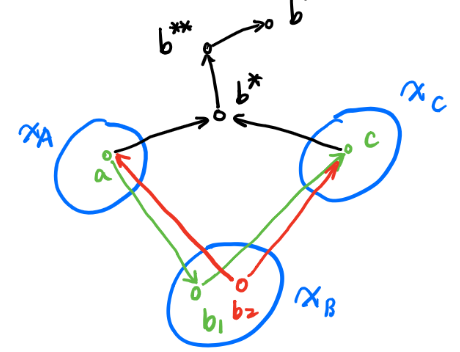
\includegraphics[width=.55\textwidth]{微信图片_20191125143139.png}
    \caption{节点之间的拓扑联系图}
    \label{fig:my_label_1}
\end{figure}

根据上一小节我们的讲解,我们可以想想,假如从$a$到$c$中间通过一个节点$b$,那么路径什么时候是连通的?什么时候又是阻塞的呢?我们可以分两种情况来讨论,为什么是两种?上一节我们就已经讲解过,Tail to Tail结构和Head to Tail结构其实是一样的,但是Head to Head结构是反常的。所以我们就分开进行讨论。

1. 如果是Tail to Tail结构和Head to Tail结构,那么中间节点$b_1,b_2$必然要位于可观测集合$X_B$中,那么$a$和$c$才是相互独立的。

2. 如果是Head to Head结构,那就不一样了,在一般情况下$a\bot c$,那就是$b\notin X_B$,包括他的子节点都不可以被观测到,不然就连通了。

如果,符合上述两条规则,那么我们就可以称$a$和$c$之间是D-Separation的,实际上还有一个名字,叫做全局马尔科夫性质 (Global Markov Property)。D-Separation非常的关键,我们可以直接用这个性质来检测两个集合关于另外一个集合被观测的条件是不是条件独立。

\section{Markov Blanket}
Markov Blanket听着像是一个很神奇的东西呀,我看着似乎也很神奇,这到底是个什么玩意呢?大家看我的分析。

我们首先定义$x_{-i}$为$\{x_1,x_2,\cdots,x_{i-1},x_{i+1},\cdots,x_N\}$,这个序列中唯独不包括$x_i$。那么,我们假设除了$x_i$节点,其他节点都是可观测的,那么我们需要计算概率:
\begin{equation}
    p(x_i|x_{-i}) = \frac{p(x_i, x_{-i})}{p(x_{-i})} = \frac{p(x)}{\int_{x_i}p(x)dx_i} = \frac{\prod_{j=1}^N p(x_j|x_{pa(j)})}{\int_{x_i}\prod_{j=1}^N p(x_j|x_{pa(j)})dx_i}
\end{equation}

我们分析一下上述等式,我们可以分成两部分,将和$x_i$相关的部分记为$\bar{\Delta}$,和$x_i$不相关的部分记为$\Delta$。那么公式(1)可以被我们改写为:
\begin{equation}
     p(x_i|x_{-i})= \frac{\Delta\cdot \bar{\Delta}}{\int_{x_i}\Delta\cdot \bar{\Delta}dx_i} = \frac{\Delta\cdot \bar{\Delta}}{\Delta\cdot \int_{x_i} \bar{\Delta}dx_i} = = \frac{ \bar{\Delta}}{ \int_{x_i} \bar{\Delta}dx_i}
\end{equation}

我们可以将$p(x_i|x_{-i})$表示为一个函数$f(\bar{\Delta})$。那么$x_i$和其他所有点的关系可以被化简为只和$x_i$相关的点的关系。那么,我们将这个关系大致抽象出来,通过图来进行分析,找一找哪些节点是和$x_i$相关的,直观性也是概率图模型的一大优点。假设$x_i$是可以被观测到的
\begin{figure}[H]
    \centering
    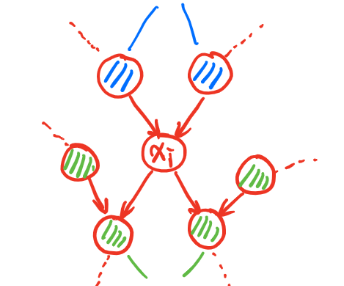
\includegraphics[width=.55\textwidth]{微信图片_20191125153322.png}
    \caption{节点之间的抽象拓扑联系图}
    \label{fig:my_label_1}
\end{figure}

$P(x_i|x_{-1})$首先包括一部分为$p(x_i|x_{pa(i)})$,第二部分为$p(x_{child(i)}|x_i,x_{pa(child(x_i))})$。为什么第二部分可以这样写呢?首先$x_i$作为两个父亲节点,得到两个孩子节点,毫无疑问对吧,那么我们可以写成$p(x_{child(i)}|x_i)$。但是和$p(x_{child(i)})$相关的变量除了$x_i$肯定还有其他的,也就是$x_{pa(child(x_i))}$,所以我们就可以得到$p(x_{child(i)}|x_i,x_{pa(child(x_i))})$。

实际上,这些$x_i$周围的节点,也就是我用阴影部分画出的那些,可以被称为Markov Blanket。从图上看就是留下和父亲,孩子,孩子的另一个双亲,其他的节点可以忽略,也就是和周围的关系的连接。

~\\

我这里关于概率图和条件独立性有一点的懵逼,我梳理一下思路。D-Separation是在概率图中,帮助我们快速的判断条件独立性。对于一个节点,它和哪些节点相关,它和和父亲,孩子,孩子的另一个双亲这三种节点相关,这三种点的集合就是Markov Blanket。在概率图中,我们用$p(x_1,x_2,\cdots,x_N)=\prod_{i=1}^Np(x_i|x_{pa\{i\}}$和$p(x_1,x_2,\cdots,x_N)=p(x_i)\prod_{i=1}^Np(x_i|x_{1:i-1})$两种表达形式是等价的。第二种事最完备的表达方法,第一种的表达是简化版本,他蕴含了概率图中得到的条件独立性关系简化的结果。我不知道,我这样解释这几个概念之间的关系怎么样?有更好的建议,欢迎批评指正,请通过gongchen2020@ ia.ac.cn联系我。
























\end{document}
